\documentclass[11pt]{article}

\usepackage[a4paper,margin=1in]{geometry}
\usepackage{amsmath,amssymb}
\usepackage{booktabs}
\usepackage{microtype}
\usepackage{xcolor}
\usepackage{pgfplots}
\pgfplotsset{compat=1.17}
\usepgfplotslibrary{groupplots}
\usepackage{titlesec}
\usepackage[hidelinks]{hyperref}

% --- HELIX accent palette (muted, professional) ---
\definecolor{accent}{RGB}{15,110,86}   % teal 600
\definecolor{amber}{RGB}{186,117,23}    % amber 600
\definecolor{coral}{RGB}{153,60,29}     % coral 800
\definecolor{rule}{RGB}{180,178,169}    % gray 200

\titleformat{\section}{\color{accent}\large\bfseries}{\thesection}{0.6em}{}
\titleformat{\subsection}{\color{accent!85!black}\normalsize\bfseries}{\thesubsection}{0.6em}{}

\newcommand{\dcor}{\mathrm{dCor}}
\newcommand{\dcov}{\mathrm{dCov}}
\newcommand{\E}{\mathbb{E}}
\newcommand{\KL}{D_{\mathrm{KL}}}

% boxed summary
\newcommand{\keybox}[1]{%
  \begin{center}\fcolorbox{accent}{accent!6}{%
  \begin{minipage}{0.93\linewidth}\vspace{4pt}#1\vspace{4pt}\end{minipage}}\end{center}}

\title{\vspace{-2.2em}\color{accent}\bfseries
Pearson vs.\ Distance Correlation for ABCD Background Estimation}
\author{\normalsize Nathan Herling \\[-2pt]
\small UA ATLAS HEP Group \,$\cdot$\, Project HELIX \,$\cdot$\, Run~3 LLP MSVtx search}
\date{\small\today}

\begin{document}
\maketitle
\vspace{-1.2em}
\hrule height 1.2pt \vspace{1em}

\noindent
We are testing whether the two NN discriminants used in the ABCD background
estimate behave as statistically independent variables. The natural first
instinct is to report a Pearson correlation; the measured value is
$\rho \approx 0.3$. This note argues that Pearson is the wrong statistic for
the question being asked, that distance correlation (dCor) is the right one,
and that the failure of Pearson here is not incidental but \emph{structural}:
the properties of NN discriminants are precisely those that void Pearson's
guarantees. Three parts follow --- (1) what the two metrics measure and how
they differ, (2) the dependence each can detect that the other cannot, and
(3) why this experiment is inherently a dCor problem.

\keybox{\centering
\textbf{One line for the meeting:} Pearson can only \emph{fail to find}
dependence; dCor can \emph{certify its absence}. ABCD's null hypothesis is
independence, so we need the statistic that certifies absence.}

\section{The two metrics and their differences}

\subsection*{Pearson --- linear, signed, Gaussian-bound}
The Pearson coefficient is the normalised covariance of the raw values,
\begin{equation}
\rho \;=\; \frac{\operatorname{Cov}(X,Y)}{\sigma_X\,\sigma_Y}
      \;=\; \frac{\E\!\big[(X-\mu_X)(Y-\mu_Y)\big]}{\sigma_X\,\sigma_Y}\, .
\end{equation}
Geometrically it is the cosine of the angle between the two mean-centred data
vectors --- a single inner product. It therefore answers exactly one question:
\emph{when $X$ rises above its mean, does $Y$ rise proportionally, along a
straight line?} It is cheap, bounded in $[-1,1]$, and \emph{signed} (it reports
the direction of the trend). Its defining limitation is the direction of its
guarantee:
\begin{equation}
X \perp Y \;\Longrightarrow\; \rho = 0, \qquad\text{but}\qquad
\rho = 0 \;\not\Longrightarrow\; X \perp Y .
\end{equation}
The converse holds \emph{only} under joint Gaussianity. Outside the Gaussian
world, $\rho=0$ carries no independence content.

\subsection*{Distance correlation --- nonlinear, unsigned, distribution-free}
Distance correlation discards the raw values and works on \emph{pairwise
distances}. For samples $\{X_j\}$, form the distance matrix $a_{jk}=|X_j-X_k|$
and double-centre it,
\begin{equation}
A_{jk} \;=\; a_{jk} - \bar a_{j\cdot} - \bar a_{\cdot k} + \bar a_{\cdot\cdot},
\end{equation}
and likewise $B_{jk}$ from $\{Y_j\}$. The (squared) distance covariance and the
distance correlation are
\begin{equation}
\dcov^2(X,Y) = \frac{1}{n^2}\sum_{j,k} A_{jk}B_{jk},
\qquad
\dcor(X,Y) = \frac{\dcov(X,Y)}{\sqrt{\dcov(X,X)\,\dcov(Y,Y)}}\,\in[0,1].
\end{equation}
The question it asks is geometric: \emph{when two events are far apart in $X$,
are they also far apart in $Y$?} That is the definition of dependence itself,
and it is blind to whether the relationship is a line, a curve, a fork, or a
ring. The double-centring is the load-bearing step --- it is what makes the
key property hold for \emph{any} distribution:
\begin{equation}
\dcor(X,Y) = 0 \;\Longleftrightarrow\; X \perp Y .
\end{equation}

\subsection*{Side by side}
\begin{center}
\renewcommand{\arraystretch}{1.25}
\begin{tabular}{@{}lll@{}}
\toprule
& \textbf{Pearson $\rho$} & \textbf{Distance correlation} \\
\midrule
Built from        & raw values (covariance)        & pairwise distances \\
Detects           & linear association only        & any dependence \\
Range             & $[-1,1]$, \emph{signed}        & $[0,1]$, magnitude only \\
Zero means        & no \emph{linear} trend         & \emph{independence} (always) \\
Independence test & valid only if jointly Gaussian & valid for any distribution \\
Cost              & $O(n)$                         & $O(n^2)$ (subsample for large $n$) \\
\bottomrule
\end{tabular}
\end{center}

\noindent
A useful unifying fact: \emph{under} joint Gaussianity, dCor is a deterministic
monotonic function of $|\rho|$ --- the two carry the same information in that
regime. They disagree precisely to the extent the data departs from Gaussian.
The gap between them is itself a non-Gaussianity meter.

\section{What each can catch that the other cannot}

The detectable-dependence relation \emph{nests}:
\begin{equation}
\rho \neq 0 \;\Longrightarrow\; \dcor > 0,
\qquad\qquad
\dcor = 0 \;\Longrightarrow\; \rho = 0 .
\end{equation}
Everything Pearson can flag, dCor also flags --- plus an entire class
(nonlinear and higher-moment dependence) that Pearson cannot. As an
independence detector, Pearson's coverage is a strict subset of dCor's. The one
thing dCor lacks is the \emph{sign}: it reports how much dependence, never which
direction. For a factorisation test that asymmetry is exactly the right
trade --- we care whether dependence exists, not its sign.

\subsection*{The canonical miss: zero $\rho$, total dependence}
Let $X$ be symmetric about its mean and $Y=(X-\tfrac12)^2$. Then $Y$ is
\emph{completely determined} by $X$, yet the left and right halves contribute
opposite-sign covariance and cancel: $\rho=0$ exactly. dCor is large. Pearson
would issue a clean bill of health on a pair that ABCD cannot close. The figure
below shows the three regimes that matter.

\begin{center}
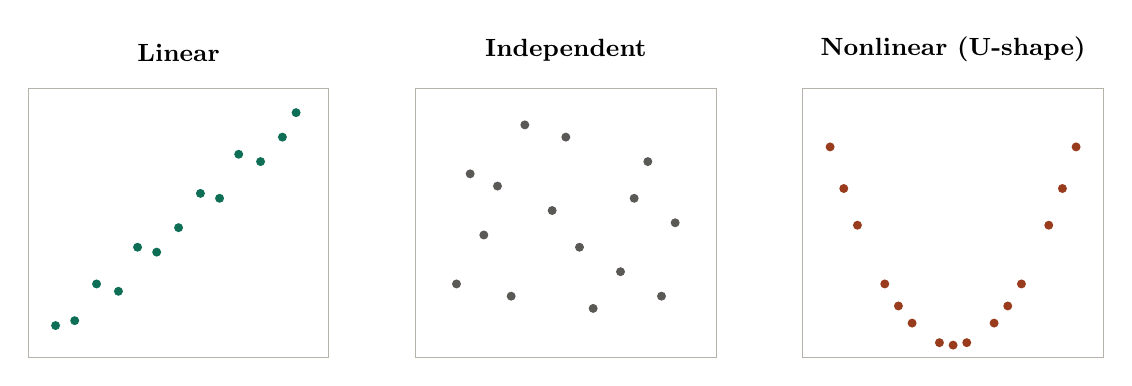
\begin{tikzpicture}
\begin{groupplot}[
  group style={group size=3 by 1, horizontal sep=1.1cm},
  width=5.4cm, height=5.0cm,
  xmin=-0.05,xmax=1.05,ymin=-0.05,ymax=1.05,
  xtick=\empty, ytick=\empty,
  axis line style={rule}, tick style={rule},
  scatter/use mapped color={draw=mapcol,fill=mapcol},
  title style={font=\bfseries\small},
]
\nextgroupplot[title={Linear}]
\addplot[only marks,mark=*,mark size=1.4pt,color=accent] coordinates {
(0.05,0.08)(0.12,0.10)(0.2,0.25)(0.28,0.22)(0.35,0.40)(0.42,0.38)(0.5,0.48)
(0.58,0.62)(0.65,0.60)(0.72,0.78)(0.8,0.75)(0.88,0.85)(0.93,0.95)};
\nextgroupplot[title={Independent}]
\addplot[only marks,mark=*,mark size=1.4pt,color=rule!50!black] coordinates {
(0.15,0.70)(0.30,0.20)(0.50,0.85)(0.20,0.45)(0.70,0.30)(0.45,0.55)(0.80,0.75)
(0.60,0.15)(0.35,0.90)(0.90,0.50)(0.10,0.25)(0.55,0.40)(0.75,0.60)(0.25,0.65)(0.85,0.20)};
\nextgroupplot[title={Nonlinear (U-shape)}]
\addplot[only marks,mark=*,mark size=1.4pt,color=coral] coordinates {
(0.05,0.81)(0.10,0.64)(0.15,0.49)(0.25,0.25)(0.30,0.16)(0.35,0.09)(0.45,0.01)
(0.50,0.00)(0.55,0.01)(0.65,0.09)(0.70,0.16)(0.75,0.25)(0.85,0.49)(0.90,0.64)(0.95,0.81)};
\end{groupplot}
\end{tikzpicture}
\end{center}
\vspace{-0.4em}
\begin{center}\small
\begin{tabular}{@{}lccc@{}}
\toprule
 & Linear & Independent & Nonlinear (U) \\
\midrule
Pearson $\rho$ & $0.95$ & $\approx 0.02$ & $\approx 0.00$ \\
dCor           & $0.95$ & $\approx 0.04$ & $0.52$ \\
Verdict        & agree  & agree          & \textcolor{coral}{\textbf{diverge --- Pearson blind}} \\
\bottomrule
\end{tabular}
\end{center}

\noindent
The two metrics agree when the relationship is linear (left) and agree when the
variables are independent (centre). They diverge only on nonlinear dependence
(right) --- and that is exactly the regime our discriminants live in.

\subsection*{The silent miss: variance dependence}
Even if the conditional \emph{mean} $\E[Y\mid X]$ is flat in $X$ (so
$\rho\approx0$), the conditional \emph{spread} $\operatorname{Var}(Y\mid X)$ can
depend strongly on $X$. NN confidence is heteroscedastic across input space
almost always. Pearson is blind to second-moment dependence; dCor catches it,
because changing spread changes pairwise distances. ABCD assumes the \emph{full}
conditional factorises, not merely the conditional mean --- so variance
dependence breaks closure while Pearson reports zero. This is the most easily
overlooked failure mode and is worth probing explicitly with a sliced scan.

\section{Why our experiment is inherently dCor}

\subsection*{The ABCD null \emph{is} an independence statement}
The ABCD prediction $A_{\text{pred}} = B\,C/D$ is exact if and only if the
background joint factorises in the two discriminants,
$P(x,y)=P(x)\,P(y)$. That is the definition of independence. So ``does ABCD
close?'' and ``are the discriminants independent in the background?'' are the
same question --- and only dCor answers it with a guarantee. Pearson can return
a comforting $0$ on a background that will not close; dCor cannot.

\subsection*{The information-theoretic identity (HELIX / MaxEnt view)}
The factorised joint $P(x)P(y)$ is exactly the maximum-entropy distribution
consistent with the two marginals: if all we constrain are $P(x)$ and $P(y)$,
Jaynes' principle returns the product as the least-committal joint. The deviation
from that null is the mutual information, and it is an identity, not an analogy:
\begin{equation}
I(X;Y) \;=\; \KL\!\big(P(x,y)\,\|\,P(x)P(y)\big),
\qquad I(X;Y)=0 \;\Longleftrightarrow\; X\perp Y .
\end{equation}
Mutual information \emph{is} the distance from the MaxEnt null; dCor is its
well-behaved, estimator-friendly cousin sharing the iff-independence property.
This is why Pearson is disqualified at the level of principle, not merely
performance: it does not measure distance from the factorised null, so it cannot
be the correct statistic even in principle. If a correlation constraint is added
to the marginals, MaxEnt returns a single exponential tilt
$P(x,y)\propto P(x)P(y)\,e^{\lambda g(x,y)}$, with $\lambda=0$ recovering
closure --- which turns any residual non-closure into a measurable parameter
(future work; the proof target).

\subsection*{Why NN1 and NN2 leave the Gaussian box}
Pearson's independence guarantee requires joint Gaussianity. NN discriminants
violate that assumption through several independent channels at once:

\begin{itemize}
\itemsep2pt
\item \textbf{Shared-latent nonlinearity.} Both networks read the same event
      (same displaced MS vertex, same kinematics). Two different nonlinear
      functions of a common cause generically produce nonlinear, often
      non-monotone dependence --- the curvature Pearson cannot see.
\item \textbf{Output squashing.} A classifier score lives in $[0,1]$ and piles
      up against the rails; the joint clusters in the corners of the plane, far
      from a Gaussian ellipse. A sigmoid output is the first thing to leave the
      Gaussian box.
\item \textbf{Tail co-movement.} The ABCD signal region is a high-score
      \emph{corner} --- a tail, not the bulk. Variables can be linearly
      uncorrelated overall yet co-move in the tails. Pearson is bulk-weighted and
      dilutes exactly the region that decides closure.
\item \textbf{Heteroscedasticity.} Confidence spread varies across input space;
      second-moment dependence is invisible to $\rho$ (see \S2).
\item \textbf{Barrel quantization.} Integer-valued inputs place the score on a
      discrete lattice --- maximally non-Gaussian, with flat-then-jump structure
      at the cut boundaries. This is the signature of the barrel $1.79$
      non-closure. (Caveat: quantization also biases dCor/MI estimation, so
      evaluate on the \emph{continuous} pre-quantization scores.)
\end{itemize}

\keybox{Each bullet is a way of being non-Gaussian, and non-Gaussian is exactly
where $\rho=0$ stops meaning independent. The discriminants violate the
assumption through \emph{several} channels simultaneously --- so it is not that
Pearson \emph{might} mislead here; the setting is built to make it mislead. dCor
evaluates them correctly because its zero is an independence certificate
regardless of distributional shape.}

\subsection*{Practical recipe}
On \emph{background-only}, \emph{continuous} scores: (i) global dCor with a
permutation test for significance; (ii) sliced dCor across NN1 to localise where
the dependence lives; (iii) the bootstrapped ABCD closure ratio as the physics
arbiter. Pearson may be reported alongside, but only as a non-Gaussianity
cross-check --- never as the basis for the independence decision.

\vspace{0.6em}
\hrule height 0.5pt
\vspace{0.4em}
{\footnotesize\itshape Honest qualifier: the arguments above establish why the
independence assumption cannot be made for these variables, not that the
dependence is necessarily large. Which channel dominates --- tail, variance, or
quantization --- is what the sliced dCor scan and conditional-shape check are
there to determine.}

\end{document}
